\chapter{Внутритекстовая когерентность}
\label{chap:coh}

\section{Каркас вычисления когерентности}

Большинство описанных в разделе \ref{sec:toptokens} предыдущей главы подходов к оценке интерпретируемости укладываются в следующую схему:

1) Для каждой темы выбирается небольшой набор характеризующих её токенов. Как правило, это список из 10 самых вероятных её токенов, но встречаются и более сложные критерии выбора \cite{blei2009topic}\cite{ldavis2014}\cite{boydcare}\cite{frex}; традиционно такие наборы называются \textit{верхними токенами} (top-tokens) данной темы.

2a) Этот набор демонстрируется человеку-эксперту, который каким-либо образом оценивает качество темы

или

2b) Для каждого элемента этого набора собирается ряд статистик совстречаемостей, на основе которого вычисляются какие-либо численные показатели

Эта схема впервые появилась во влиятельных работах Бли \cite{rtl} \cite{mrtl} и Мимно \cite{mimno2011}, а затем была существенно доработана исследовательским сообществом. Мы будем называть данное семейство метрик \textit{основанным на верхних токенах}.

Главное достоинство этих метрик заключается в их простоте. Вместо того чтобы изучать распределение вероятностей целиком, исследователю достаточно посмотреть на короткий список самых ``характерных'' слов.

Более того, благодаря работам \cite{mrtl}, \cite{mimno2011}, \cite{aletras2013evaluating}, \cite{roder2015exploring}, эта процедура может быть автоматизирована, что позволяет оптимизировать когерентность напрямую \cite{4keys}.

Однако именно из этой простоты вытекает их фундаментальное ограничение. Список из 5-10 слов не может отражать распределение вероятностей целиком (ситуация усугубляется тем, что исследователи часто игнорируют вероятности топ-слов или даже их порядок в теме).

Кроме того, по этому списку нельзя делать выводы о том, насколько хорошо тематическая модель описывает конкретную коллекцию документов. Распространена рекомендация базировать статистику совстречаемости на внешнем корпусе (например, «Википедия»); опять же, это может не отражать специфику конкретной коллекции (например, юридических текстов).

Мы утверждаем, что при помощи короткого списка топ-слов невозможно обосновать качество тематической модели (каким бы образом этот список ни анализировался). Это относится и к оценкам, полученным из рук людей-экспертов, и к величинам, вычисленным на основе совстречаемостей слов. Иными словами, критический изъян кроется в пункте (1) вышеописанной схемы, в котором тема целиком огрубляется до конечного числа слов.

\section{Критика метрик, основанных на топ-токенах}

 
  \begin{figure}[h]
  \small
  \begin{subfigure}[t]{0.39\textwidth}
    $\mbox{A}\ \mbox{group}\ \mbox{of}\ \textcolor{my-red}{astronomers}\ \mbox{managed}$\\
    $\mbox{to}\ \textcolor{my-pink}{detect} \mbox{a}\ \mbox{\textcolor{my-red}{star}},\ \mbox{\textcolor{my-pink}{orbiting}}$\\ $\mbox{\textcolor{my-pink}{around}}\ \mbox{the}\ \mbox{\textcolor{my-red}{black}}\ \mbox{\textcolor{my-red}{hole}}\ \mbox{at}$\\
    $\mbox{a}\ \mbox{very}\ \mbox{close}\ \mbox{\textcolor{my-pink}{distance}}.$
  \end{subfigure}
  ~
  \small
  \begin{subfigure}[t]{0.39\textwidth}
  $\mbox{Over}\ \mbox{the}\ \mbox{course}\ \mbox{of}\ \mbox{a}\ \mbox{single}\ \mbox{busy}\ \mbox{week,}\ \mbox{I}\ \mbox{was}\ \mbox{invited}\ \mbox{to}\ \\ \mbox{an}\ \mbox{\textcolor{my-red}{astronomers'}}\ \mbox{conference},\ \mbox{I}\ \mbox{had}\ \mbox{interviewed}\ \\
  \mbox{a}\ \mbox{famous}\ \mbox{pop}\ \mbox{\textcolor{my-red}{star}},\ \mbox{I}\ \mbox{wrote}\ \mbox{an}\ \mbox{opinion}\ \mbox{piece}\ \\
  \mbox{about}\ \mbox{\textcolor{my-red}{black}}\ \mbox{community}\ \mbox{and}\ \mbox{contributed}\ \\ \mbox{to}\ \mbox{an}\ \mbox{editorial}\ \mbox{on}\ \mbox{a}\ \mbox{\textcolor{my-pink}{massive}}\ \mbox{budget}\ \mbox{\textcolor{my-red}{hole}}.$
  \end{subfigure}
  
  \vspace{0.35cm}
  
  \[
  t = \mbox{Black Holes} = 
      \{\mbox{\textcolor{my-red}{black}}, \mbox{\textcolor{my-red}{hole}}, \mbox{\textcolor{my-red}{star}},
      \mbox{\textcolor{my-red}{astronomer}}, \mbox{\textcolor{my-pink}{orbiting}}, 
      \mbox{\textcolor{my-pink}{distance}}, \mbox{\textcolor{my-pink}{detect}},
      \mbox{\textcolor{my-pink}{massive}}, \ldots\}
  \]
  
  \caption{
      An example illustrating why top-tokens based coherences may act badly in some cases.
      In the two presented pieces of text words related to the topic "Black Holes" are coloured (red~---~strongly related to the topic, pink~---~partially related).
      Text on the left is "good", it is actually about black holes.
      On the other hand, right text is nonsense.
      However, these texts are organized in a way to leave the top tokens of the topic "Black Holes" (red words) on nearly the same places in the text, i.e. if some of these tokens appeared in one words window on the left, so as on the right.
      Top-tokens based coherences would feel no difference.
      New intra-text measures should sense that something is "wrong" with text on the right, it is not connected with the topic.
  }
  \label{plot:ideal-tm}
\end{figure}

Для того чтобы обосновать это заявление, мы опишем ряд проблем, присущих всем критериям качества, основанным на верхних токенах.

\subsection{Учёт специфики коллекции}

Автоматизированные метрики когерентности основываются на счётчиках совстречаемости слов. Общая идея таких процедур состоит в следующем:

1) подсчитывается, сколько раз определённые слова оказываются внутри одного и того же скользящего окна (контекста); иногда контекстом может выступать весь документ целиком.

2) полученное число сравнивается с частотой, предсказанной в предположении о том, что все совстречаемости случайны.

Если случайное совпадение не может объяснить имеющиеся статистики совместной встречаемости слов, то тема называется \textit{когерентной} (буквально: связной, цельной, согласованной). Таким образом, когерентность определяется через позиции слов: тема называется когерентной, если её слова встречаются кластерами, а не разбросаны по документам случайно.

Ориентирующийся на когерентность исследователь неявно рассуждает таким образом:
\begin{enumerate}
    \item Верхние токены темы имеют высокую когерентность
    \item Верхние токены темы встречаются в документах согласованным образом
    \item Все токены темы встречаются в документах согласованным образом
    \item Тема является хорошей
\end{enumerate}

Переход от (1) к (2) может быть проблематичным, если статистика совстречаемостей подсчитывается на основании внешнего корпуса (например, «Википедии»), а лексика в исследуемой коллекции текстов используется в специфичных значениях или употребляется нетипичным образом.

Переход от (2) к (3) некорректен по другой причине: происходит вывод о качестве темы в целом на основе поведения десяти её самых частых слов (подобные рассуждения уже критиковались в работе  \cite{dh_sea}). Неэквивалентность утверждений ``верхние 10 слов темы когерентны'' и ``вся тема когерентна'' можно показать численно. Более подробно это будет подсчитано в секции \ref{sec:represented}

% However, our preliminary estimations indicate that the real frequency tend to be dramatically lower (around $0.03\%$ for individual topic).

\subsection{Топ-токены и хвосты распределения}

\dscl{Этому аргументу не хватает конкретных чисел. Возможно, даже с числами будет не совсем убедительно, насколько это может быть вредно на самом деле; может быть надо просто брать не топ-10 слов, а отсекать по суммарному порогу}

Из определения топ-слов следует, что они не отражают информацию, содержащуюся в хвостах распределения $\phi_{wt}$ (например, список топ-слов не изменится, если обнулить вероятности всех слов, кроме 10 наиболее частых).

Это может приводить к ошибочным рассуждениям. Например, в уже упомянутой работе~\cite{wang2016catching} делается вывод о том, что самой ``любимой'' темой читателей Трампа является тема \texttt{Демократы}. Здесь делается неявное допущение о том, что тема эквивалентна понятию, объединяющему множество её топ-слов. Похожее допущение принимается и при изучении графика ``вероятность темы в момент времени'', как в работе \cite{monsters_men, dispatch}.

Для того чтобы сделать это рассуждение более строгим, мы измерим следующее: 1) как изменится распределение $\theta_{td}$, если обнулить хвосты распределения (то есть: отражают ли пропорции $\theta_{td}$ частоты топ-слов темы); 2) какова вероятность встретить топ-слово темы $t$ в теме $t'$ и как это зависит от регуляризации (то есть: насколько можно ``спрятать'' часть тематических слов внутри других тем).

% \subsection{Когерентность как показатель улучшения}

% как когерентность должна выглядеть на графиках "когерентность vs номер итерации". Там должны быть резкие скачки и периоды "стабильности". Математическая интуиция говорит о том, что когерентность должна меняться только в те моменты, когда какое-либо слово вошло в топ-10 или вышло из него, и меняться она при этом должна резкими скачками.

% token ordering

% hence it changes only when some token leaves the top10 list to be replaced by another token.

% when they switch places

% The issue is mitigated somewhat by averaging.
% If we average within the large number of topics
% Even better,
% you can restart the inference of topic model several times from different initializations.

% However, this is flawed when researcher is interested in a single topic.
\todo{Про то, что множество топ-слов когерентнее чем специфиная тема}

\subsection{Когерентность и стоп-слова}

В работе \cite{fan2019assessing} приводится критика когерентности, основанная на рассуждениях другого характера. Сначала отмечается, что стоп-слова могут быть каноничными (``the'' и ``and'' для английского языка) или специфическими для данной области (``ребёнок'' и ``сын'' для корпуса педагогической направленности).

Работа со стоп-словами --- важный шаг, которому редко уделяется должное внимание. В частности, распространена практика итерационного построения LDA с обновлением списка стоп-слов (в который попадают неинформативные верхние слова из модели, построенной ранее). В работе \cite{boydcare} упоминается сходная рекомендация. В пример приводится тема, верхние токены которой состоят из римских чисел: vii, viii, xiv, xiii, xii и т.д. К сожалению, этот подход снижает объективность и воспроизводимость результатов.

В связи с этим в работе \cite{fan2019assessing} подчёркивается и экспериментально подтверждается проблема мер когерентности в условиях наличия стоп-слов. Меры когерентности, основанные на документной совстречаемости, ``поощряют'' присутствие в теме частых неинформативных токенов, поскольку такие токены часто встречаются в одном и том же документе. В результате корреляция
этих показателей качества с экспертными оценками интерпретируемости существенно снижается, когда в верхних словах темы имеются стоп-слова. Кроме того, когерентность не позволяет проконтролировать различность тем.

Описываемое явление действительно встречалось в нашей практике при построении тематической модели над корпусом 20NG \ref{fig:law_gun_would}.

\begin{table}[t]
    \caption{10 верхних слов в двух темах и оценки их качества при помощи UMass-когерентности и UCI-когерентности. Первая тема более интерпретируема, при этом численные оценки отмечают её низкую когерентность.}
    \label{fig:law_gun_would}
    \small
    \begin{tabular}{ | p{7.5cm}| p{3.5cm} |p{3.5cm} |}
    \hline
    Верхние слова &  UMass & UCI
    \\ \hline	
law gun state government right weapon crime bill firearm control &
-2.2584 & 0.7389
    \\ \hline
one would get go say think make time know like & \textbf{-0.9392} & \textbf{0.7822}
    \\ \hline
    \end{tabular}
\end{table}

\section{Эксперимент: никаких оценок без представительства}
\label{sec:represented}


\begin{figure}
    %\begin{tabular}{p{7.5cm}p{3.5cm}}
        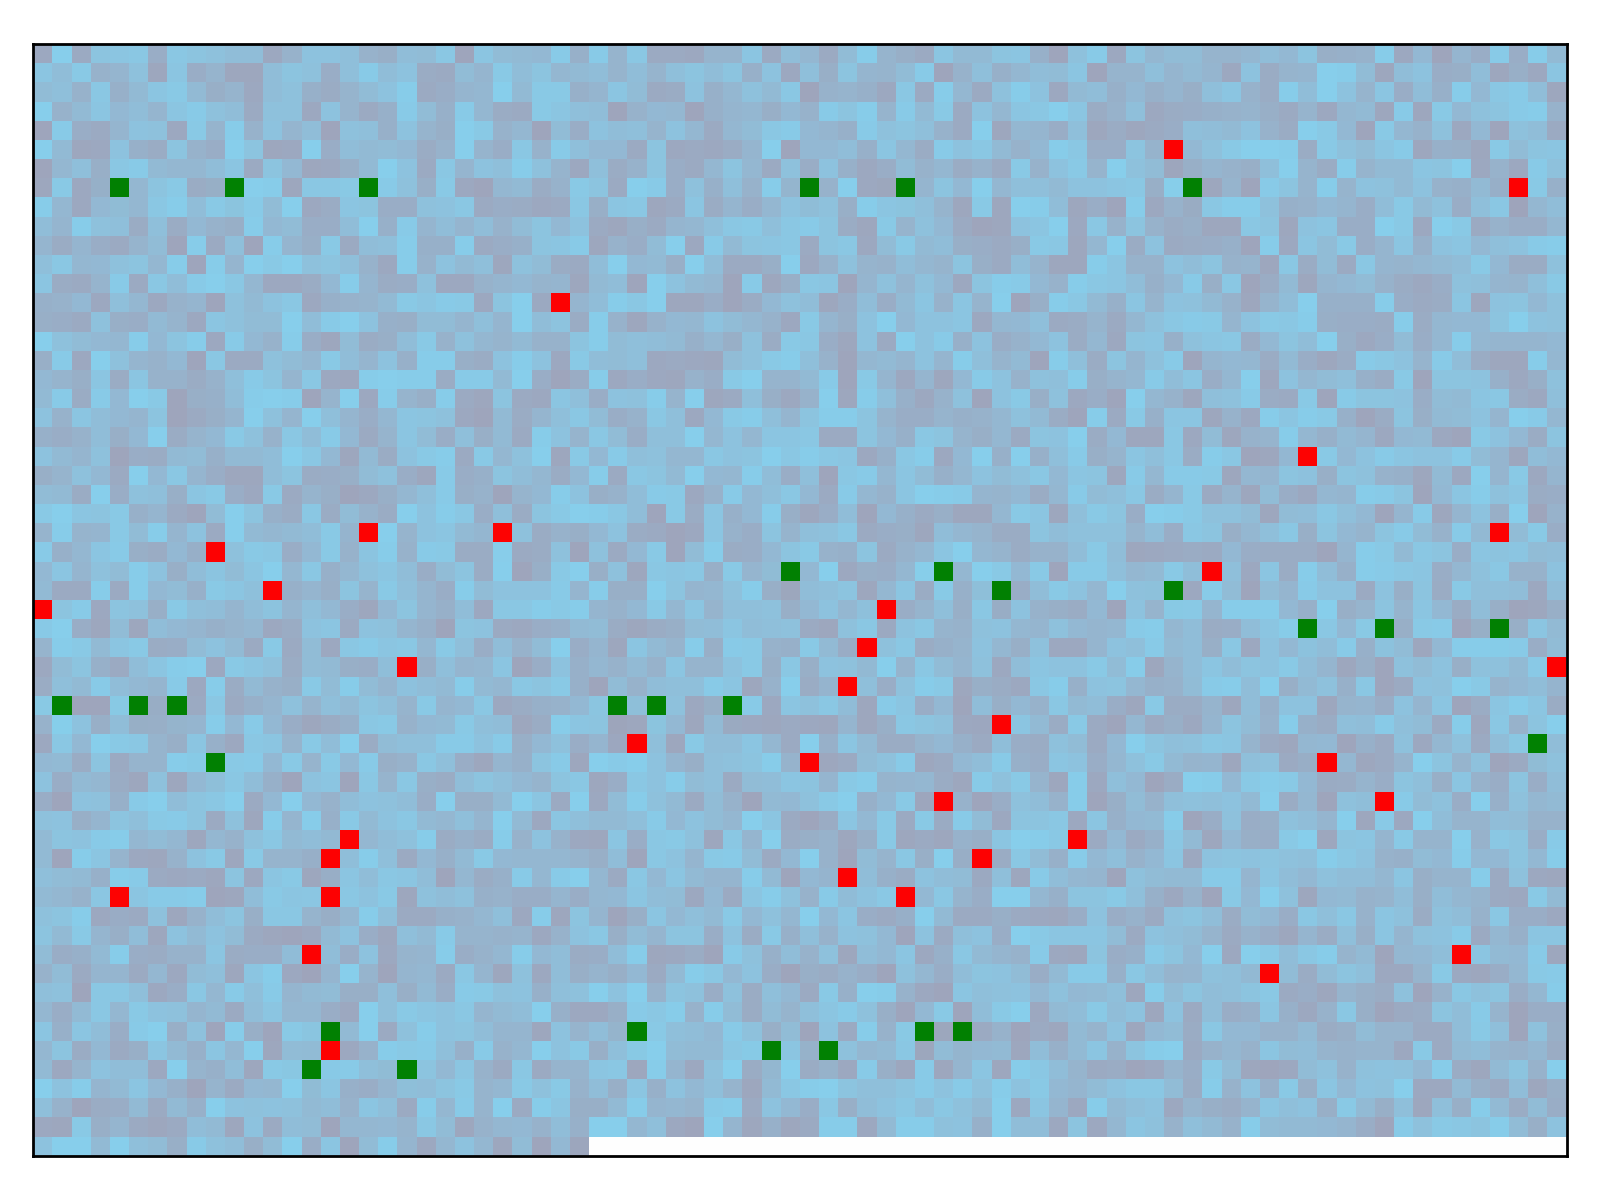
\includegraphics[width=0.75\textwidth]{doc11358_topic0.png} %&
        % 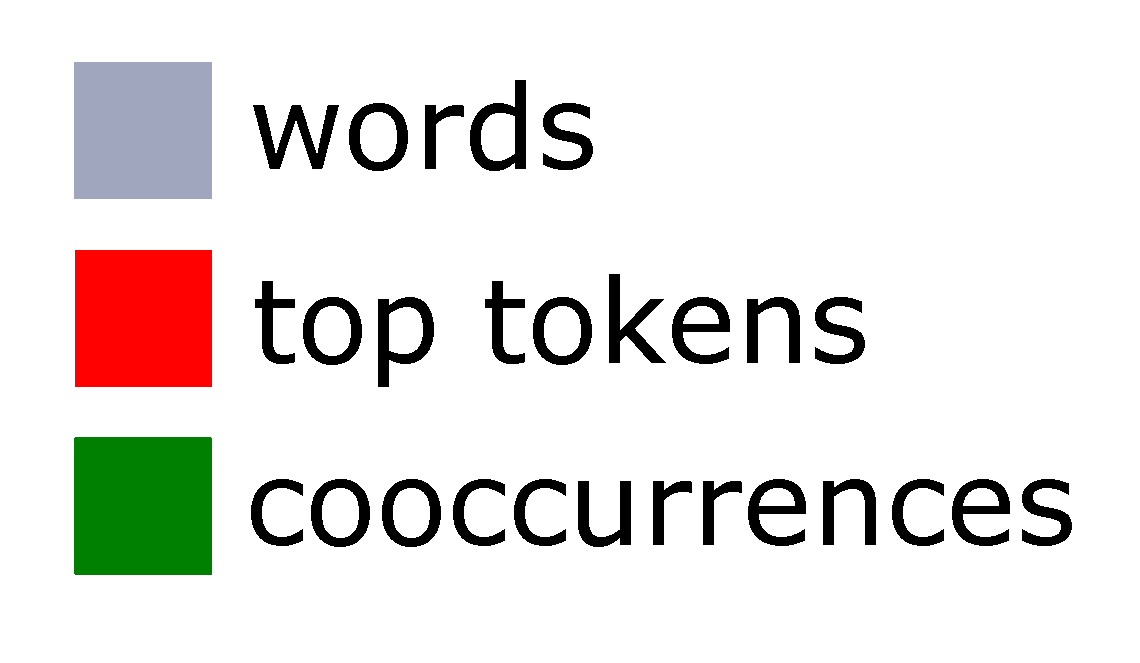
\includegraphics[width=0.25\textwidth]{legend.eps} \\
    %\end{tabular}
    \caption{Демонстрация доли текста, покрытой верхними словами, на примере одного документа. Словопозиции обозначены серо-синим цветом, словопозиции верхних слов показаны красным цветом, зелёным цветом показаны словопозиции, имеющие ненулевой вклад в расчёт когерентности (т.е. попадающие в скользящее окно вместе с другим верхним словом).}
\label{fig:ch3_doc_compound}
\end{figure}


Пусть $Q$ --- некое множество слов. Эти слова встречаются в некоем документе $d$, который можно считать списком словопозиций: $d = [w_1, w_2, w_3, \dots w_{n_1}]$.

Назовём словопозицию $i, ~w_i \in Q$ \textit{представленной}, если существует какое-либо контекстное окно $[w_i, w_{i+1}, w_{i+2}, \dots w_{i+k-1}, w_{i+k}]$, содержащее эту позицию вместе с позицией какого-либо другого слова $v, v \in Q$. Таким образом, словопозиция является \textit{представленной} если и только если у неё ненулевой вклад в счётчики совстречаемости множества $Q$.

Теперь можно сформулировать следующий естественный вопрос: если совстречаемости посчитаны на основе 10 топ-слов одной темы (или сразу нескольких тем), то какая доля словопозиций коллекции \textit{представлена} в этих статистиках?

Ясно, что эта величина не может быть больше, чем общая частота топ-слов в коллекции (эта частота обычно лежит в промежутке $1\%$ - $5\%$).

\dscl{тут стоит расширить эксперименты, посмотреть больше моделей (в том числе и с разной регуляризацией)}
\dscl{Мне кажется, что тут не хватает двух экспериментов. 1) Представительность нужно посмотреть с другим размером множества топ-токенов (не 10, а 20, 30, 50, 100; отсечение по порогу, а не по константе).}

Мы измерим представительность двух тематических моделей на двух разных коллекциях документов. Первая модель построена на коллекции статей сайта ``ПостНаука'' и состоит из 19 предметных и одной фоновой темы. Вторая модель является наиболее интерпретируемой (согласно людям-экспертам, оценивавшим 10 топ-слов тем) из 9 моделей, рассмотренных в работе~\cite{rtl}. Эта модель построена на подвыборке статей английской «Википедии» и состоит из 50 тем.

\begin{table}[ht]
\begin{tabular}{lll}
         & ПостНаука & Википедия \\
Минимум  & 0.0159\%  & 0.0065\%  \\
Медиана  & 0.0483\%  & 0.0293\%  \\
Среднее  & 0.0619\%  & 0.0356\%  \\
Максимум & 0.2764\%  & 0.1149\%  \\
Суммарно & 1.2027\%  & 1.6585\%
\end{tabular}
    \caption{
      Доля коллекции, имеющая ненулевой вклад в счётчики совстречаемости 10 топ-слов. Статистики посчитаны по каждой теме отдельно; строка ``суммарно'' показывает представительность объединённого множества топ-слов всех тем.
    }
    \label{table:represented}
\end{table}

Как можно видеть в таблице \ref{table:represented}, топ-слова покрывают исчезающе малую часть коллекции (менее 2\% корпуса). Когерентность отдельно взятой темы в большинстве случаев учитывает менее тысячной доли всего корпуса текста.


\section{Предлагаемая мера: внутритекстовая когрентность}

Как было замечено ранее, традиционные метрики когерентности неявно основываются на допущении о том, что слова ``хороших'' тем часто встречаются рядом. Это похоже на лингвистическую концепцию \textit{когезии} \cite{halliday1976cohesion}: предложения естественного языка подчинены линейной внутренней структуре. Эта горизонтальная структура организуется
различными синтаксическими и лексическими средствами: союзами, повторами, словами-заместителями, согласованием временных и иных форм \cite{kazachenko2009}.

В данной работе делается предположение, что тексты естественного языка состоят из связных фрагментов, каждый из которых содержит малое число скрытых тем. Из этого следует, что интерпретируемость темы должна оцениваться не как согласованность наиболее частых слов темы, но как согласованность слов темы внутри связных фрагментов текста. Нужно заметить, что частая совместная встречаемость самых вероятных слов тоже косвенно указывает на то, что тема встречается в текстовой коллекции как связный фрагмент текста.

При помощи этого рассуждения можно построить семейство автоматизированных мер интерпретируемости. Каждая из них будет измерять, насколько ``быстро'' или ``сильно'' меняется тематический профиль соседних слов.

Таким образом, мы меняем порядок вычислений когерентности. Традиционные меры когерентности сначала выделяют какое-то множество слов по их $\phi_{wt}$ и затем анализируют, каким образом эти слова встречаются в тексте (\emph{от темы к тексту}). В предлагаемом же методе сначала выделяются все соседние слова текста, распределение $\phi_{wt}$ которых затем анализируется (\emph{от текста к теме}).

Можно предложить несколько принципиально разных подходов к формализации этой идеи.





\begin{figure}
  \small
  \begin{tabularx}{1.0\textwidth}{l| *{3}{Y}|*{3}{Y}|}
    & \multicolumn{3}{c|}{Low variance}
    & \multicolumn{3}{c|}{High variance}\\
    \cline{2-7}
    & русский & поэт & Пушкин & Толстой & Рассел & Эйлер \\
    \begin{tabular}[c]{@{}l@{}}$\begin{smallmatrix}\\ \textcolor{my-red}{Literature} \\\\
    \textcolor{green}{Philosophy} \\\\
    \textcolor{blue}{Mathematics} \\\\
    \end{smallmatrix}$\end{tabular}  &
    \begin{tabular}[c]{@{}l@{}}
      $\smalltopicvector{my-red!50}{green!25}{blue!25}$
    \end{tabular} &
    \begin{tabular}[c]{@{}l@{}}
      $\smalltopicvector{my-red!90}{green!10}{blue!10}$
    \end{tabular} &
    \begin{tabular}[c]{@{}l@{}}
      $\smalltopicvector{my-red!90}{green!10}{blue!10}$
    \end{tabular} &
    \begin{tabular}[c]{@{}l@{}}
      $\smalltopicvector{my-red!90}{green!30}{blue!10}$
    \end{tabular} &
    \begin{tabular}[c]{@{}l@{}}
      $\smalltopicvector{my-red!10}{green!50}{blue!50}$
    \end{tabular} &
    \begin{tabular}[c]{@{}l@{}}
      $\smalltopicvector{my-red!10}{green!10}{blue!90}$
    \end{tabular}
  \end{tabularx}
    \caption{Caption}
    \label{fig:intracohs_pic1}
\end{figure}
\textbf{Средний разброс в окне.} Семантическую близость расположенных рядом слов можно выразить как дисперсию векторов с компонентами $p(t \cond w)$ (см. \ref{fig:intracohs_pic1}). Данная величина подсчитывается в каждом скользящем окне длиной в $p_1$ слов. Другая естественная вариация --- среднее попарное расстояние векторов $p(t \cond w)$ в скользящем окне. Расстояние можно подсчитывать несколькими способами (например, как евклидово расстояние или как косинусную близость).

\begin{figure}
    \noindent
    $\mbox{Группе}\ \underbrace{\mbox{\textcolor{my-pink}{астрономов}}\ \mbox{удалось}}_{l_1=2}\ \mbox{обнаружить}\ \underbrace{\mbox{\textcolor{my-pink}{звезду}}, \mbox{обращающуюся}}_{l_2=2}$\\
    $\mbox{вокруг}\ \underbrace{\mbox{\textcolor{my-red}{чёрной}}\ \mbox{\textcolor{my-red}{дыры}}\ \mbox{на}\ \mbox{рекордно}\ \mbox{близком}}_{l_3=4}\ \mbox{расстоянии}.$
    \caption{Пример. Тема $t = \mbox{``Чёрные дыры''}$}
    \label{fig:intracohs_pic3}
\end{figure}

\textbf{Длина сегмента.} Другим показателем тематической однородности может быть средняя продолжительность темы внутри текста. Будем считать, что слово $w$ относится к теме $t$, если разность между компонентой вектора $p(t \cond w)$, отвечающей теме $t$, и максимальной компонентой из оставшихся больше заданного порога (здесь в качестве порога был использован $0$).

На практике оказывается нужен дополнительный механизм, уменьшающий чувствительность меры качества к словам общей лексики. Для этого можно ``разрешить'' ей учитывать чуждые текущей теме слова с небольшим негативным штрафом. Когда величина суммарно набранного штрафа пересекает заданный порог, сегмент отмечается как закончившийся; количество отмеченных слов и будет значением искомой метрики качества (см. \ref{fig:intracohs_pic3}).

\begin{figure}
    \centering
    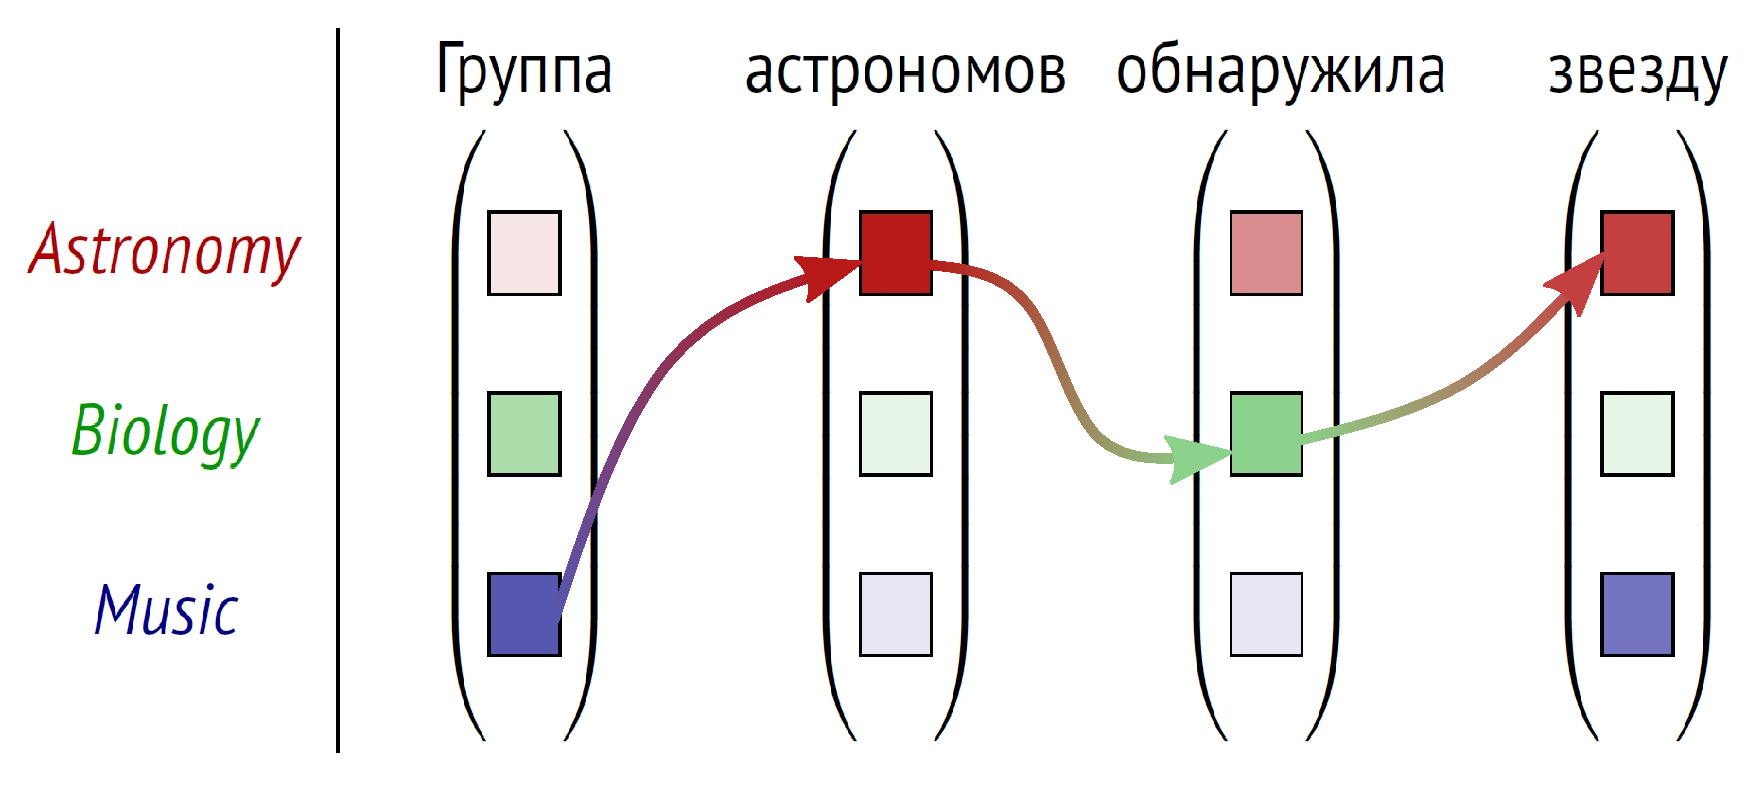
\includegraphics[width=0.8\textwidth, height=0.2\textheight]{astronomers_focon.eps} % .eps image is wrong scaled
    \caption{Caption}
    \label{fig:intracohs_pic2}
\end{figure}

\textbf{Скачки тематики.} Третий подход к измерению внутритекстовой когерентности --- оценивать, как сильно в целом по всему тексту отличаются по тематике смежные слова. Суммируются попарные разности между максимальными вероятностями в каждом векторе $p(t\mid w)$. Подразумевается, что наиболее вероятные темы у соседних слов могут различаться, но тема не должна ``затухать'' слишком быстро (см. \ref{fig:intracohs_pic2}).

Этот подход также требует механизма работы с ``чуждыми'' словами: два слова считаются соседними, если количество принадлежащих фоновой теме слов между ними не больше заданного порога (фоновой считается тема, имеющая больше всего приписанных к ней словопозиций в данном документе).

\section{Постановка задачи}

Оценка интерпретируемости --- очень трудоёмкое мероприятие, даже для процедур, основанных на топ-словах.
В данной работе эта проблема усугубляется. С одной стороны, мы желаем построить меру качества, учитывающую $\Phi$, $\Theta$ и коллекцию документов целиком. С другой стороны, валидация такой метрики требует сравнения её с человеческими оценками интерпретируемости (что означает необходимость разметки огромного массива данных).

Мы предлагаем способ обойтись без этого затруднительного мероприятия: вместо того, чтобы размечать данные вручную, можно сгенерировать полусинтетический корпус с известной разметкой. Структура коллекции «ПостНаука» играет в этом важную роль: темы статей настолько обширны и различны, что большинство документов являются \textit{монотематическими}: каждое слово такого документа связано не более чем с одной предметной темой (иными словами, монотематические документы --- это документы, все слова которых являются либо фоновыми, либо относятся к определённой предметной теме). Среди 3446 оригинальных статей исходной коллекции 2118 являются монотематическими.

Полусинтетическая коллекция будет собрана из фрагментов таких монотематических документов. Исходные тексты разбиваются на сегменты, которые перемешиваются и объединяются в новые документы.

% Идея состоит в том, что большие монотематические документы можно разрезать на маленькие монотематические сегменты, которые затем будут случайно сшиты вместе.

В результате этого процесса получается коллекция данных с известным общим числом тем, распределением тем в документах и даже известными метками тем для слов. Отметим, что любая тематическая модель неявно классифицирует слова заданного документа по темам. Действительно, любому слову $w$ из документа $d$ соответствует величина $p_{tdw} = p(t \mid d, w \propto \phi_{wt}\theta_{td}$, задаваемая тематической моделью. Таким образом, полусинтетическая коллекция позволяет определить эталонную меру качества произвольной тематической модели, измеряя соответствие между $p_{tdw}$ и ''эталонной'' меткой слова $w$. Назовём эту меру \textit{качеством сегментации} данной тематической модели.

Качество сегментации текста тематической моделью оценивается ``мягким'' образом: для каждой темы $t$ считается сумма $p(t \mid d, w)$ на всех парах $(d, w),\ d \hm\in D,\ w \hm\in W_d$, итоговый результат~---~сумма таких сумм по всем темам. Для того чтобы вычислить указанные выше величины, необходимо знать соответствие между темами, выданными моделью, и темами исходного датасета статей ``ПостНауки''. Для этого использовался венгерский алгоритм, выдающий наиболее удачное соответствие тем модельная-исходная.

Искомый процесс оценки различных мер качества будет построен следующим образом. Пусть дано множество различных тематических моделей. Для каждой модели можно вычислить её качество сегментации и различные рассматриваемые меры качества (как традиционные меры когерентности, так и предлагаемые меры внутритекстовой когерентности). Таким образом, каждой модели $m_i$ можно сопоставить набор численных значений $f_j(m_i)$ --- замеры её качества при помощи различных методов $f_j$. Величина, которая будет показывать качество какого-либо из методов --- коэффицент корреляции Спирмана между $f_j(m_i)$ и качеством сегментации $m_i$ по всем возможным $m_i$.

В данной работе мы ставим задачу показать, что в серии моделей с улучшающейся интерпретируемостью внутритекстовые меры когерентности монотонно возрастают, в то время как способы оценки когерентности по верхним словам этого не делают.

\section{Вычислительный эксперимент}

\begin{figure}[h]

    \centering
    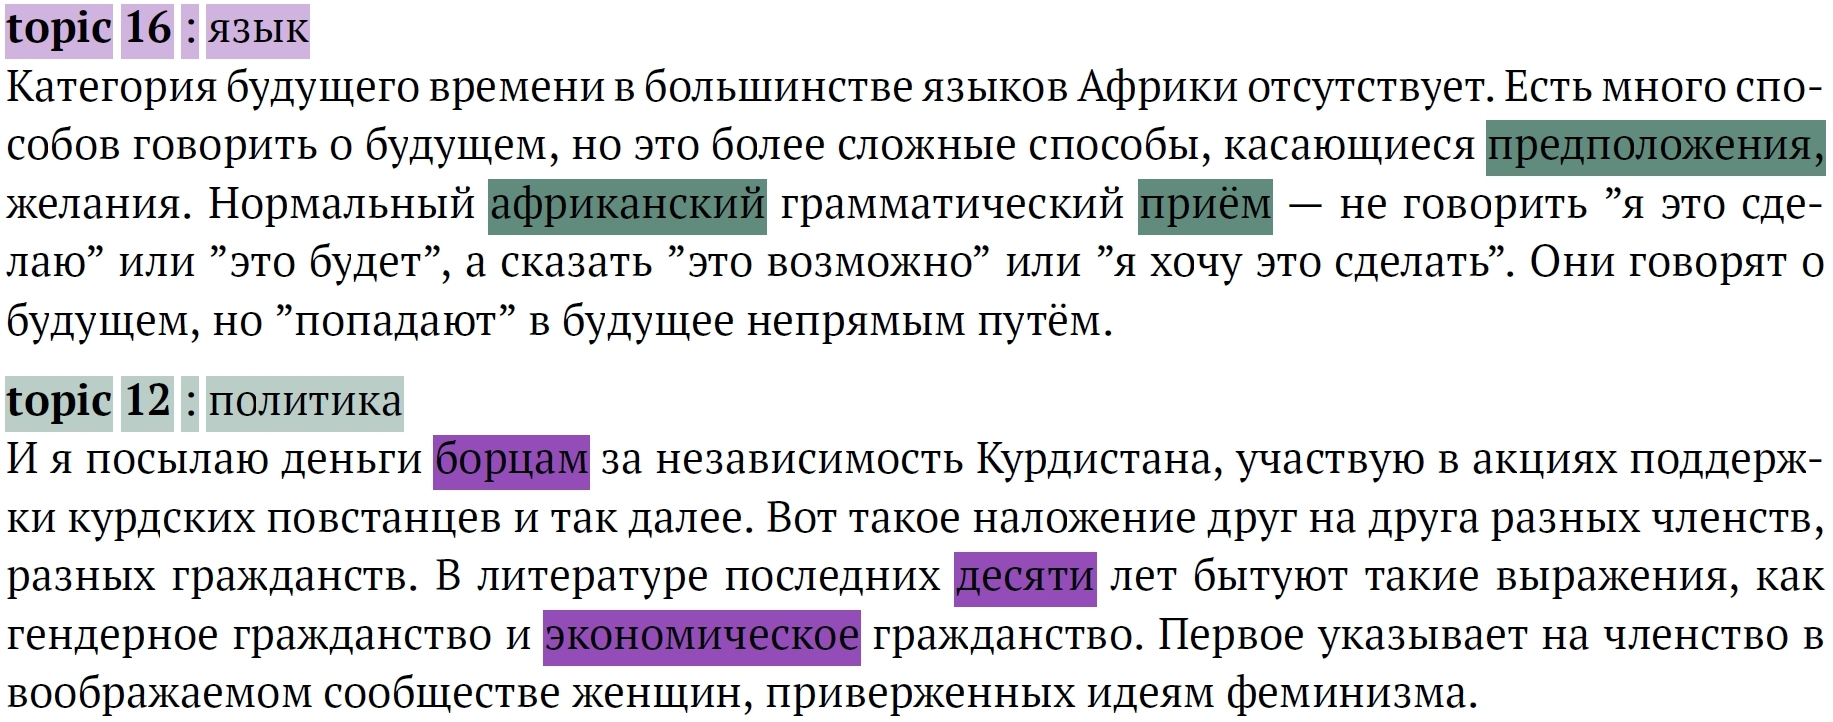
\includegraphics[width=\textwidth]{combine_bad.jpg}

  \vspace{-0.5cm}

    \scriptsize
    \centering
    \begin{tabular}{rrrrrrrrr}
      SQ (S) & SQ (H) & N & M & SC L2 & SC Cos & SC Var & TL & FC\\
      \midrule
      \rowcolor{my-blue-light}
      5500 & 11000 & -4.8 & -3.1 & -13 & 0.95 & -37000 & 2.9 & -140000\\
      \textbf{16000} & \textbf{38000} & \textbf{-3.7} & \textbf{-2.7} & \textbf{-3.7} & 0.70 & \textbf{-8100} & \textbf{3.5} & \textbf{-54000}
    \end{tabular}

  \begin{itemize}\setlength{\itemindent}{0pt}
    \small
    \item SQ (S), SQ (H)~---~Soft and Strict segmentation qualities
    \item N, M~---~Newman, Mimno
    \item SC, TL, FC~---~SemantiC, TopLen, FoCon
  \end{itemize}

    \centering
    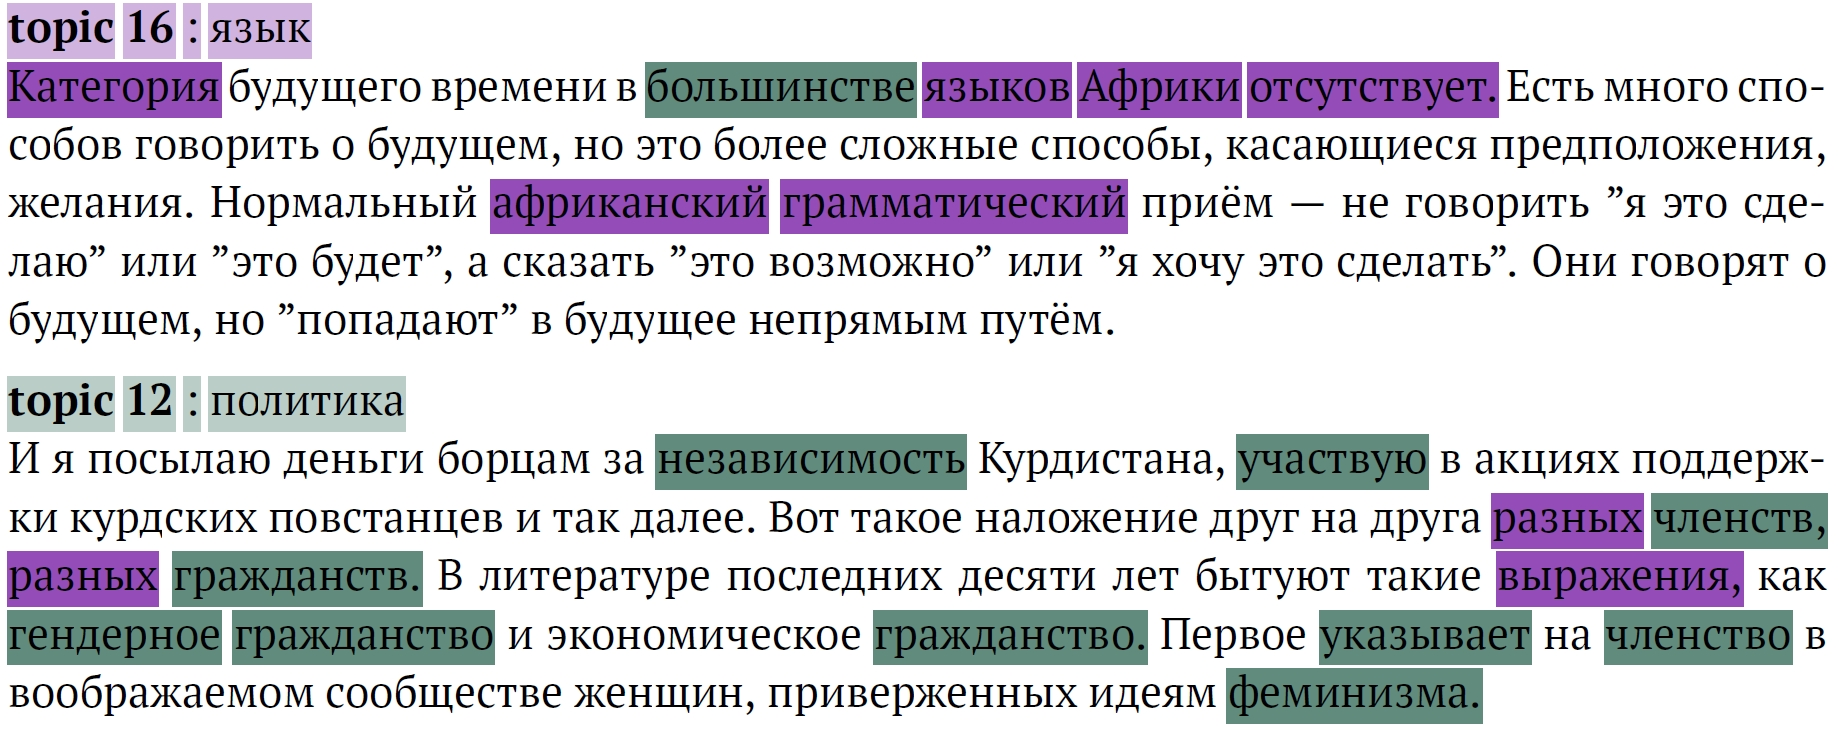
\includegraphics[width=\textwidth]{combine_good.jpg}

  \vspace{-0.5cm}

    \scriptsize
    \centering
    \begin{tabular}{rrrrrrrrr}
      SQ (S) & SQ (H) & N & M & SC L2 & SC Cos & SC Var & TL & FC\\
      \midrule
      5500 & 11000 & -4.8 & -3.1 & -13 & 0.95 & -37000 & 2.9 & -140000\\
      \rowcolor{my-blue-light}
      \textbf{16000} & \textbf{38000} & \textbf{-3.7} & \textbf{-2.7} & \textbf{-3.7} & 0.70 & \textbf{-8100} & \textbf{3.5} & \textbf{-54000}
    \end{tabular}

  \begin{itemize}\setlength{\itemindent}{0pt}
    \small
    \item SQ (S), SQ (H)~---~Soft and Strict segmentation qualities
    \item N, M~---~Newman, Mimno
    \item SC, TL, FC~---~SemantiC, TopLen, FoCon
  \end{itemize}

    \label{fig:segm_good_bad}
    \caption{Рисунок показывает фрагмент одного из сгенерированных документов, который состоит из двух соседних сегментов различных тем длиной 50 слов. Слова сегментов обработаны описанными ранее ``хорошей'' моделью и ``плохой'' моделью. Нераскрашенные слова были отнесены к какой-либо теме, отличной от двух ``главных''. Также приведены численные величины различных когерентностей и значения, характеризующие качество сегментации. Полужирным отмечены ситуации, в которых значение когерентности возрастает при улучшении качества модели.}
\end{figure}



\begin{figure}
    \centering
    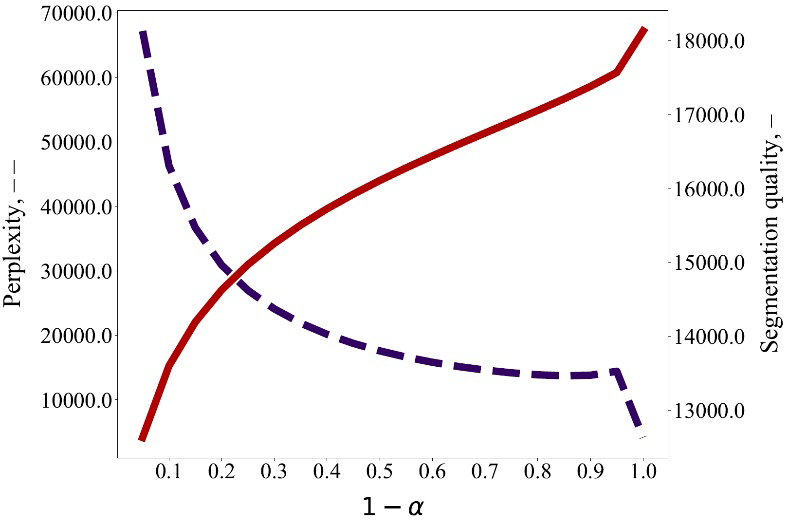
\includegraphics[width=0.8\textwidth]{images/segm_1.png}
    \caption{  На графике показана зависимость мер качества от степени деградации матрицы $\Phi$. Согласованность качества сегментации и перплексии говорит о том, что качество сегментации действительно характеризует ``хорошесть'' тематической модели.}
    \label{plot:segm_quality-iteration}
\end{figure}

График \ref{plot:segm_quality-iteration} показывает, как ведёт себя качество мягкой сегментации при увеличении внутренней меры качества тематической модели.

Выборка тематических моделей, по которой рассчитывалась корреляция Спирмана, представлет собой параметризованное параметром $\alpha$ семейство. Матрица $\Phi$ модели из этого семейства является взвешенной комбинацией

\[
m(\alpha) = \alpha \Phi_{bad} + (1-\alpha)\Phi_{good},
\]

где $\Phi_{good}$ --- матрица $\Phi$ описанной выше модели корпуса «ПостНауки», а $\Phi_{bad}$ --- набор случайных столбцов, порождённых распределением Дирихле ($0.01^{|W|}$). Были проведены четыре серии экспериментов с различными матрицами $\Phi_{bad}$. На рисунке \ref{fig:segm_good_bad} показано различие качества этих моделей на примере сегментации одного из документов.

\subsection{Результаты}
Представлены три метода оценки интерпретируемости тематических моделей: SemantiC, TopLen и FoCon. В отличие от традиционных оценок когерентности, предложенные методы пытаются учесть все словопозиции коллекции.

Для того чтобы сравнить предложенные меры качества с двумя традиционными метриками (Newman и Mimno), был проведён эксперимент на полусинтетическом датасете, составленном из сегментов различных тем.

В экспериментах анализировались корреляции между значениями когерентностей и качеством сегментации текстов. Два из предложенных методов --- SemantiC и TopLen --- и существующая метрика UMass-когерентность показывают высокие корреляции с качеством сегментации.

\begin{figure}
\begin{tabular}{cc}
    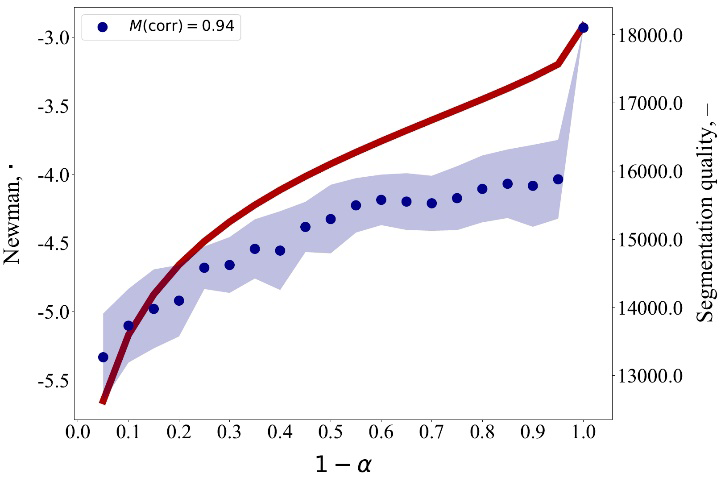
\includegraphics[width=70mm]{images/segm_mimno.png} &   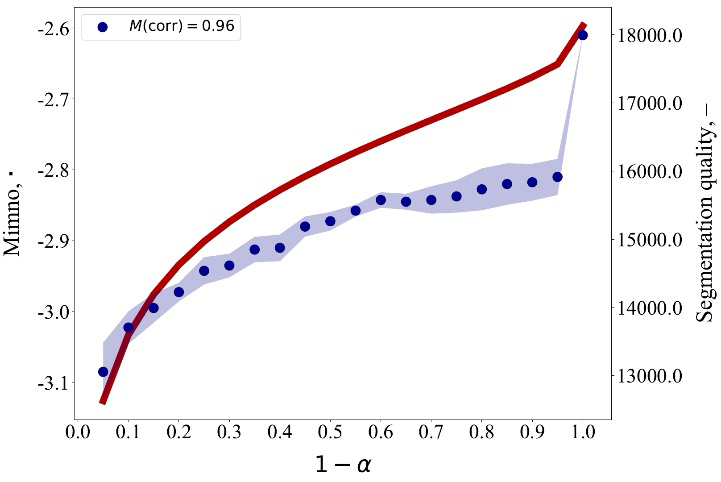
\includegraphics[width=70mm]{images/segm_newman.png} \\
 
    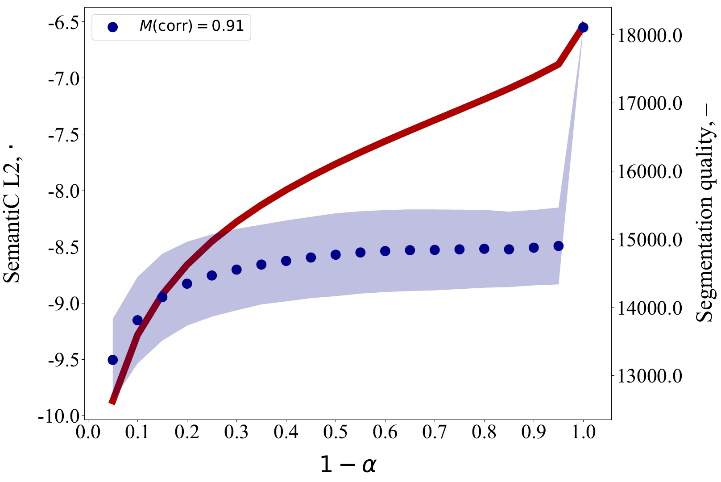
\includegraphics[width=70mm]{images/segm_l2.png} &   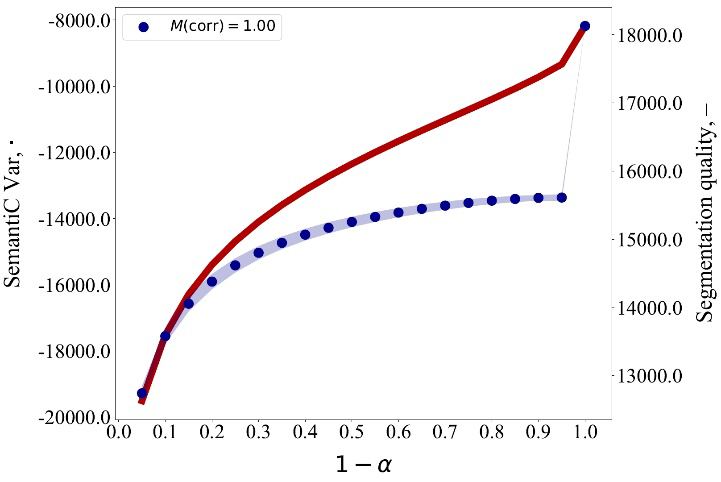
\includegraphics[width=70mm]{images/segm_var.png} \\
 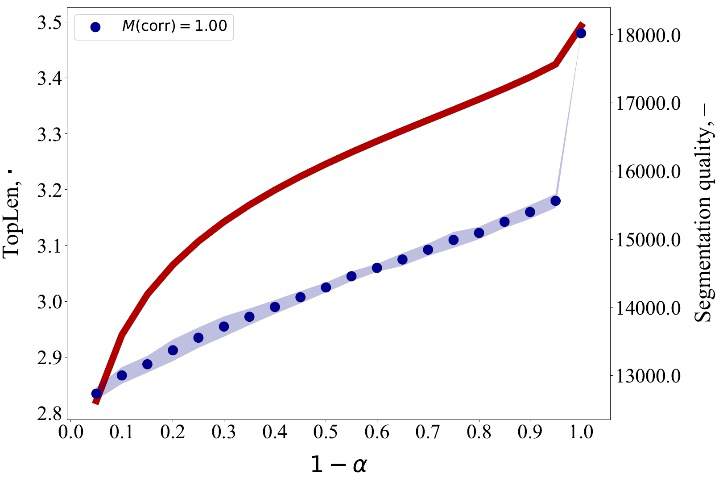
\includegraphics[width=70mm]{images/segm_toplen.png} &   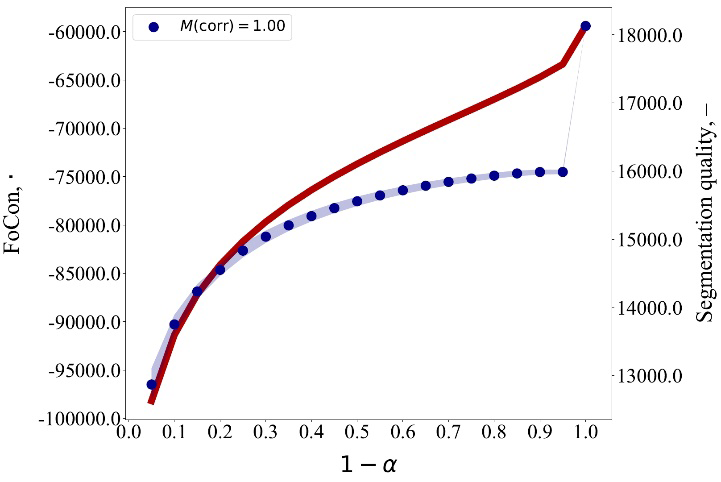
\includegraphics[width=70mm]{images/segm_focon.png} \\
\end{tabular}
    \caption{Сравнение различных мер когерентности и качества сегментации, нарисованное как функция от степени деградации тематической модели $\alpha$. }
\label{fig:ch3_corr}
\end{figure}




% SQ (S) --- мягкая segmentation quality, SQ (H)—strict segmentation quality, N—Newman, M—Mimno, SC—SemantiC, TL—TopLen, FC—FoCon.
 
